
\documentclass[letterpaper,hide notes,xcolor={table,svgnames},pdftex,10pt]{beamer}
\def\showexamples{t}


%\usepackage[svgnames]{xcolor}

%% Demo talk
%\documentclass[letterpaper,notes=show]{beamer}

\usecolortheme{crane}
\setbeamertemplate{navigation symbols}{}

\usetheme{MyPittsburgh}
%\usetheme{Frankfurt}

%\usepackage{tipa}

\usepackage{hyperref}
\usepackage{graphicx,xspace}
\usepackage[normalem]{ulem}
\usepackage{multicol}
\usepackage{amsmath,amssymb,amsthm,graphicx,xspace}
\newcommand\SF[1]{$\bigstar$\footnote{SF: #1}}

\usepackage[default]{sourcesanspro}
\usepackage[T1]{fontenc}
\usepackage[scaled]{beramono}
\usepackage{tikzpagenodes}

\newcounter{tmpnumSlide}
\newcounter{tmpnumNote}


% old question code
%\newcommand\question[1]{{$\bigstar$ \small \onlySlide{2}{#1}}}
% \newcommand\nquestion[1]{\ifdefined \presentationonly \textcircled{?} \fi \note{\par{\Large \textbf{?}} #1}}
% \newcommand\nanswer[1]{\note{\par{\Large \textbf{A}} #1}}


 \newcommand\mnote[1]{%
   \addtocounter{tmpnumSlide}{1}
   \ifdefined\showcues {~\tiny\fbox{\arabic{tmpnumSlide}}}\fi
   \note{\setlength{\parskip}{1ex}\addtocounter{tmpnumNote}{1}\textbf{\Large \arabic{tmpnumNote}:} {#1\par}}}

\newcommand\mmnote[1]{\note{\setlength{\parskip}{1ex}#1\par}}

%\newcommand\mnote[2][]{\ifdefined\handoutwithnotes {~\tiny\fbox{#1}}\fi
% \note{\setlength{\parskip}{1ex}\textbf{\Large #1:} #2\par}}

%\newcommand\mnote[2][]{{\tiny\fbox{#1}} \note{\setlength{\parskip}{1ex}\textbf{\Large #1:} #2\par}}

\newcommand\mquestion[2]{{~\color{red}\fbox{?}}\note{\setlength{\parskip}{1ex}\par{\Large \textbf{?}} #1} \note{\setlength{\parskip}{1ex}\par{\Large \textbf{A}} #2\par}\ifdefined \presentationonly \pause \fi}

\newcommand\blackboard[1]{%
\ifdefined   \showblackboard
  {#1}
  \else {\begin{center} \fbox{\colorbox{blue!30}{%
         \begin{minipage}{.95\linewidth}%
           \hspace{\stretch{1}} Some space intentionally left blank; done at the blackboard.%
         \end{minipage}}}\end{center}}%
         \fi%
}



%\newcommand\q{\tikz \node[thick,color=black,shape=circle]{?};}
%\newcommand\q{\ifdefined \presentationonly \textcircled{?} \fi}

\usepackage{listings}
\lstset{basicstyle=\footnotesize\ttfamily,
	breaklines=true,
	aboveskip=15pt,
  	belowskip=15pt,
	frame=lines,
	numbers=left, basicstyle=\scriptsize, numberstyle=\tiny, stepnumber=0, numbersep=2pt
}

\usepackage{siunitx}
\newcommand\sius[1]{\num[group-separator = {,}]{#1}\si{\micro\second}}
\newcommand\sims[1]{\num[group-separator = {,}]{#1}\si{\milli\second}}
\newcommand\sins[1]{\num[group-separator = {,}]{#1}\si{\nano\second}}
\sisetup{group-separator = {,}, group-digits = true}

%% -------------------- tikz --------------------
\usepackage{tikz}
\usetikzlibrary{positioning}
\usetikzlibrary{arrows,backgrounds,automata,decorations.shapes,decorations.pathmorphing,decorations.markings,decorations.text,decorations.pathreplacing}

\tikzstyle{place}=[circle,draw=blue!50,fill=blue!20,thick, inner sep=0pt,minimum size=6mm]
\tikzstyle{transition}=[rectangle,draw=black!50,fill=black!20,thick, inner sep=0pt,minimum size=4mm]

\tikzstyle{block}=[rectangle,draw=black, thick, inner sep=5pt]
\tikzstyle{bullet}=[circle,draw=black, fill=black, thin, inner sep=2pt]

\tikzstyle{pre}=[<-,shorten <=1pt,>=stealth',semithick]
\tikzstyle{post}=[->,shorten >=1pt,>=stealth',semithick]
\tikzstyle{bi}=[<->,shorten >=1pt,shorten <=1pt, >=stealth',semithick]

\tikzstyle{mut}=[-,>=stealth',semithick]

\tikzstyle{treereset}=[dashed,->, shorten >=1pt,>=stealth',thin]

\usepackage{ifmtarg}
\usepackage{xifthen}
\makeatletter
% new counter to now which frame it is within the sequence
\newcounter{multiframecounter}
% initialize buffer for previously used frame title
\gdef\lastframetitle{\textit{undefined}}
% new environment for a multi-frame
\newenvironment{multiframe}[1][]{%
\ifthenelse{\isempty{#1}}{%
% if no frame title was set via optional parameter,
% only increase sequence counter by 1
\addtocounter{multiframecounter}{1}%
}{%
% new frame title has been provided, thus
% reset sequence counter to 1 and buffer frame title for later use
\setcounter{multiframecounter}{1}%
\gdef\lastframetitle{#1}%
}%
% start conventional frame environment and
% automatically set frame title followed by sequence counter
\begin{frame}%
\frametitle{\lastframetitle~{\normalfont(\arabic{multiframecounter})}}%
}{%
\end{frame}%
}
\makeatother

\makeatletter
\newdimen\tu@tmpa%
\newdimen\ydiffl%
\newdimen\xdiffl%
\newcommand\ydiff[2]{%
    \coordinate (tmpnamea) at (#1);%
    \coordinate (tmpnameb) at (#2);%
    \pgfextracty{\tu@tmpa}{\pgfpointanchor{tmpnamea}{center}}%
    \pgfextracty{\ydiffl}{\pgfpointanchor{tmpnameb}{center}}%
    \advance\ydiffl by -\tu@tmpa%
}
\newcommand\xdiff[2]{%
    \coordinate (tmpnamea) at (#1);%
    \coordinate (tmpnameb) at (#2);%
    \pgfextractx{\tu@tmpa}{\pgfpointanchor{tmpnamea}{center}}%
    \pgfextractx{\xdiffl}{\pgfpointanchor{tmpnameb}{center}}%
    \advance\xdiffl by -\tu@tmpa%
}
\makeatother
\newcommand{\copyrightbox}[3][r]{%
\begin{tikzpicture}%
\node[inner sep=0pt,minimum size=2em](ciimage){#2};
\usefont{OT1}{phv}{n}{n}\fontsize{4}{4}\selectfont
\ydiff{ciimage.south}{ciimage.north}
\xdiff{ciimage.west}{ciimage.east}
\ifthenelse{\equal{#1}{r}}{%
\node[inner sep=0pt,right=1ex of ciimage.south east,anchor=north west,rotate=90]%
{\raggedleft\color{black!50}\parbox{\the\ydiffl}{\raggedright{}#3}};%
}{%
\ifthenelse{\equal{#1}{l}}{%
\node[inner sep=0pt,right=1ex of ciimage.south west,anchor=south west,rotate=90]%
{\raggedleft\color{black!50}\parbox{\the\ydiffl}{\raggedright{}#3}};%
}{%
\node[inner sep=0pt,below=1ex of ciimage.south west,anchor=north west]%
{\raggedleft\color{black!50}\parbox{\the\xdiffl}{\raggedright{}#3}};%
}
}
\end{tikzpicture}
}


%% --------------------

%\usepackage[excludeor]{everyhook}
%\PushPreHook{par}{\setbox0=\lastbox\llap{MUH}}\box0}

%\vspace*{\stretch{1}

%\setbox0=\lastbox \llap{\textbullet\enskip}\box0}

\setlength{\parskip}{\fill}

\newcommand\noskips{\setlength{\parskip}{1ex}}
\newcommand\doskips{\setlength{\parskip}{\fill}}

\newcommand\xx{\par\vspace*{\stretch{1}}\par}
\newcommand\xxs{\par\vspace*{2ex}\par}
\newcommand\tuple[1]{\langle #1 \rangle}
\newcommand\code[1]{{\sf \footnotesize #1}}
\newcommand\ex[1]{\uline{Example:} \ifdefined \presentationonly \pause \fi
  \ifdefined\showexamples#1\xspace\else{\uline{\hspace*{2cm}}}\fi}

\newcommand\ceil[1]{\lceil #1 \rceil}


\AtBeginSection[]
{
   \begin{frame}
       \frametitle{Outline}
       \tableofcontents[currentsection]
   \end{frame}
}



\pgfdeclarelayer{edgelayer}
\pgfdeclarelayer{nodelayer}
\pgfsetlayers{edgelayer,nodelayer,main}

\tikzstyle{none}=[inner sep=0pt]
\tikzstyle{rn}=[circle,fill=Red,draw=Black,line width=0.8 pt]
\tikzstyle{gn}=[circle,fill=Lime,draw=Black,line width=0.8 pt]
\tikzstyle{yn}=[circle,fill=Yellow,draw=Black,line width=0.8 pt]
\tikzstyle{empty}=[circle,fill=White,draw=Black]
\tikzstyle{bw} = [rectangle, draw, fill=blue!20, 
    text width=4em, text centered, rounded corners, minimum height=2em]
    
    \newcommand{\CcNote}[1]{% longname
	This work is licensed under the \textit{Creative Commons #1 3.0 License}.%
}
\newcommand{\CcImageBy}[1]{%
	\includegraphics[scale=#1]{creative_commons/cc_by_30.pdf}%
}
\newcommand{\CcImageSa}[1]{%
	\includegraphics[scale=#1]{creative_commons/cc_sa_30.pdf}%
}
\newcommand{\CcImageNc}[1]{%
	\includegraphics[scale=#1]{creative_commons/cc_nc_30.pdf}%
}
\newcommand{\CcGroupBySa}[2]{% zoom, gap
	\CcImageBy{#1}\hspace*{#2}\CcImageNc{#1}\hspace*{#2}\CcImageSa{#1}%
}
\newcommand{\CcLongnameByNcSa}{Attribution-NonCommercial-ShareAlike}

\newenvironment{changemargin}[1]{% 
  \begin{list}{}{% 
    \setlength{\topsep}{0pt}% 
    \setlength{\leftmargin}{#1}% 
    \setlength{\rightmargin}{1em}
    \setlength{\listparindent}{\parindent}% 
    \setlength{\itemindent}{\parindent}% 
    \setlength{\parsep}{\parskip}% 
  }% 
  \item[]}{\end{list}} 




\title{Lecture 35 --- DevOps, but Operations }

\author{Patrick Lam \& Jeff Zarnett \\ \small \texttt{patrick.lam@uwaterloo.ca} \texttt{jzarnett@uwaterloo.ca}}
\institute{Department of Electrical and Computer Engineering \\
  University of Waterloo}
\date{\today}


\begin{document}

\begin{frame}
  \titlepage

 \end{frame}


\begin{frame}
\frametitle{Devops, but Operations}

Services are doing The Thing -- but how do we know if there's a problem?

Monitoring and Alerting.

\begin{center}
	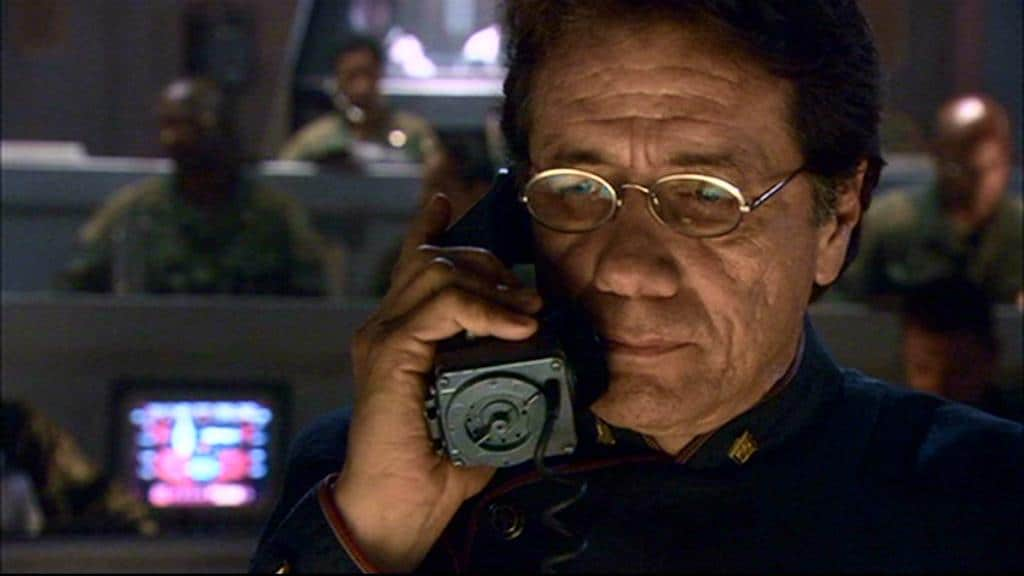
\includegraphics[width=0.8\textwidth]{images/adama.jpg}
\end{center}
``Action stations. Set Condition 1 throughout the ship!''
\end{frame}


\begin{frame}
\frametitle{What to Monitor?}

What to monitor and what to do about it?

Applications have health checks, but how basic should they be?

Maybe automate testing the basic workflow.

These don't show performance problems.

\end{frame}


\begin{frame}
\frametitle{What To Monitor, For Real?}


\begin{itemize}
	\item CPU Load
	\item Memory Utilization
	\item Disk Space
	\item Disk I/O
	\item Network Traffic
	\item Clock Skew
	\item Queue lengths
	\item Application Response Times
\end{itemize}

\end{frame}


\begin{frame}
\frametitle{Overview and Summary}

It would be good to have a dashboard of some sort.

It's a little late to recommend you take a course in the future...

Dashboards are cool but shouldn't be used to identify alerts.

\end{frame}


\begin{frame}
\frametitle{Alert Conditions}

\begin{itemize}
	\item CPU usage exceeding threshold for a certain period of time
	\item Increased rate of error logs over a period of time
	\item A service has restarted many times recently
	\item Queue length very long
	\item Taking too long to complete a workflow
\end{itemize}

\end{frame}


\begin{frame}
\frametitle{Interpreting Alerts}

\begin{center}
	
\includegraphics[width=\textwidth]{images/whyyelling.png}
\end{center}


\end{frame}




\begin{frame}
\frametitle{Sir Arthur Conan Doyle Nerdery}

\begin{center}
	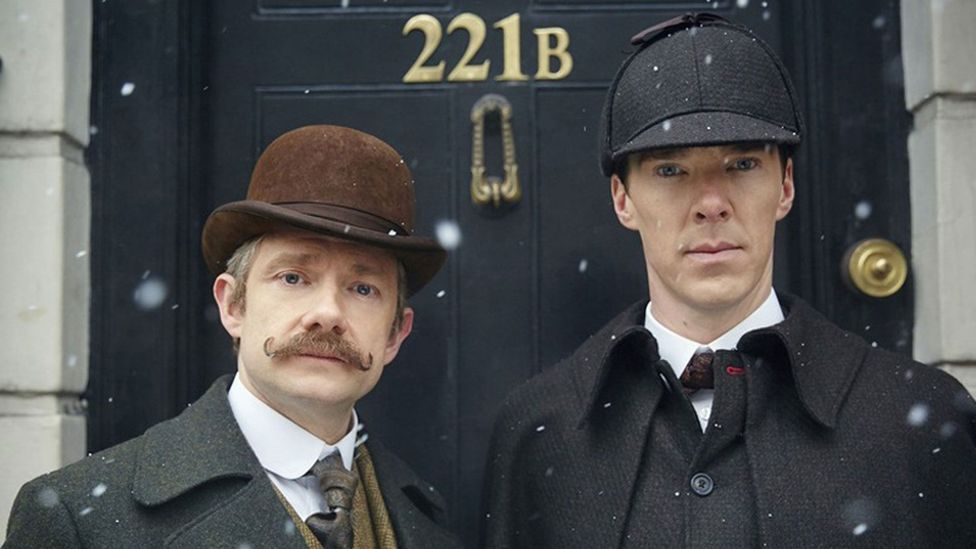
\includegraphics[width=0.8\textwidth]{images/more-sherlock.jpg}
\end{center}

Remember also the lesson from Sherlock Holmes in ``The Adventure of Silver Blaze'' -- the dog that did \alert{not} bark was a clue as to who did the crime.

\end{frame}


\begin{frame}
\frametitle{Customer Support}

The final option for detecting a problem is customer support.

Automated monitoring maybe can't find everything every time, but we shouldn't be relying on this as the primary mechanism.


\end{frame}


\begin{frame}
\frametitle{Red Alert}


\begin{itemize}
\item {\bf Alerts}: a human must take action now;
\item {\bf Tickets}: a human must take action soon \\ \qquad (hours or days);
\item {\bf Logging}: no need to look at this \\ \qquad except for forensic/diagnostic purposes.
\end{itemize}


Common bad situation: logs-as-tickets.
\end{frame}



\begin{frame}
\frametitle{Alerting}

 We usually talk about it in the metaphor of pagers, as in the small rectangular box that wakes up doctors when patients need them.
 
 \begin{center}
	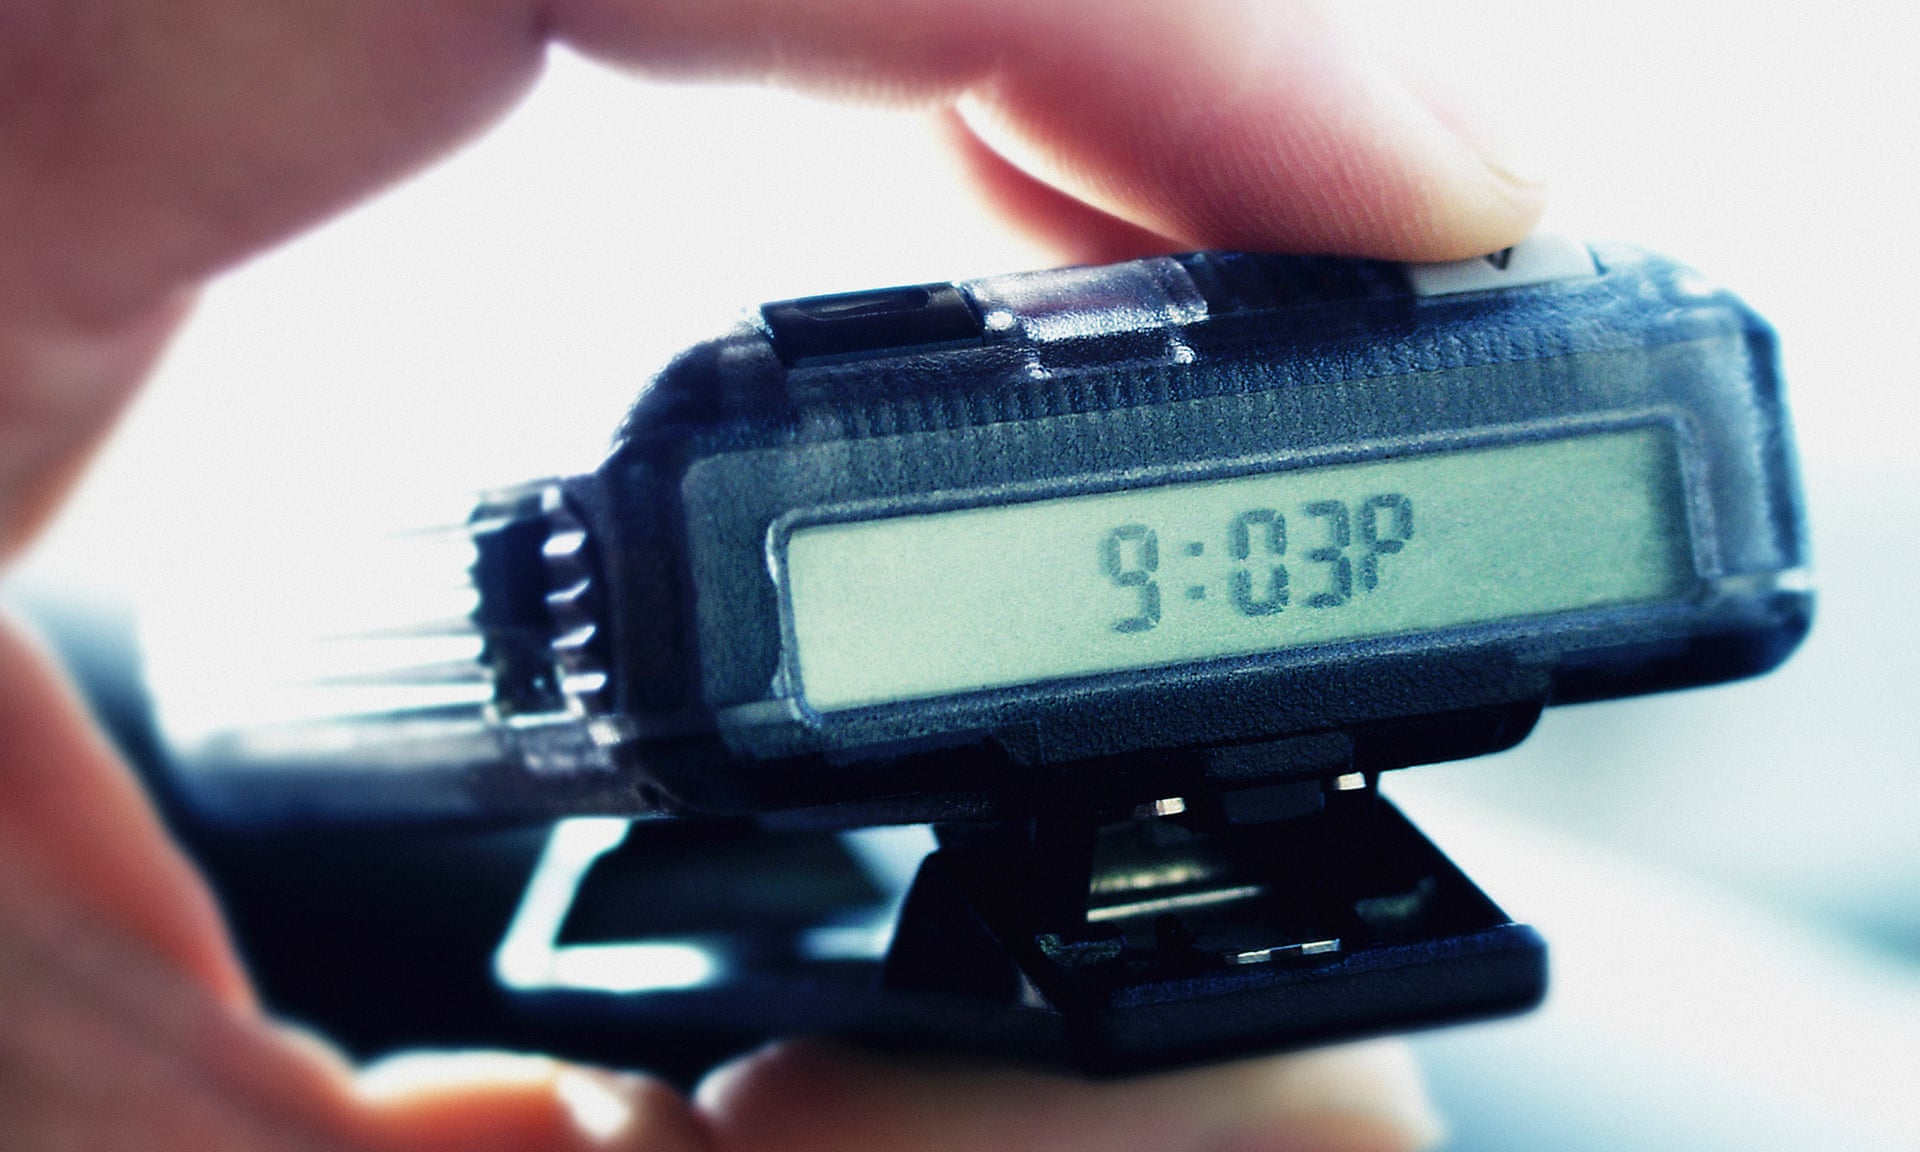
\includegraphics[width=0.4\textwidth]{images/pager.jpg}
\end{center}

The alert may contain some information about the event that has caused it.

Example: Service $A$ CPU usage is high.

\end{frame}


\begin{frame}
\frametitle{Beep Beep}

\large

What do you do when you hear the fire alarm?

\end{frame}


\begin{frame}
\frametitle{Back to Sleep}

We have experienced too many false alarms.


If there is an actual fire, you will not only be wrong, you might also be dead.
\end{frame}


\begin{frame}
\frametitle{Not the Kittens!!!}

Alerts and tickets are a great way to make user pain into developer pain.

Some SUPER CRITICAL ticket OMG KITTENS ARE ENDANGERED is an excellent way to learn the lesson... 

Devs will take steps that keep these things from happening in the future.
\end{frame}


\begin{frame}
\frametitle{Incident Reports}

Learning from incidents requires reports (post-mortems).

Identify root causes and what we can learn. 

Reports are worth doing even if they aren't fun.

\end{frame}


\begin{frame}
\frametitle{Report Content}

Breakdown of what happened with timeline.

What happened, when it was noticed, actions taken, when it was resolved.

\begin{center}
	
\includegraphics[width=0.3\textwidth]{images/just-the-facts.jpg}
\end{center}


\end{frame}


\begin{frame}
\frametitle{Root Cause Analysis}

There are two kinds of causes: root causes and proximate causes.

Example: deadlock.

How far do we go in terms of finding the root cause?

\end{frame}


\begin{frame}
\frametitle{Toyota Methodology: Five Whys}

Toyota model: ask ``why?'' five times to get to the root cause.

Does not have to be exactly 5; use judgement.

Too few times $\rightarrow$ superficial answers.

Too many times $\rightarrow$ ``computers were a mistake.''

\end{frame}


\begin{frame}
\frametitle{Action Items}

What will we do in the short term and long term?

Prevent this from happening again.

\begin{center}
	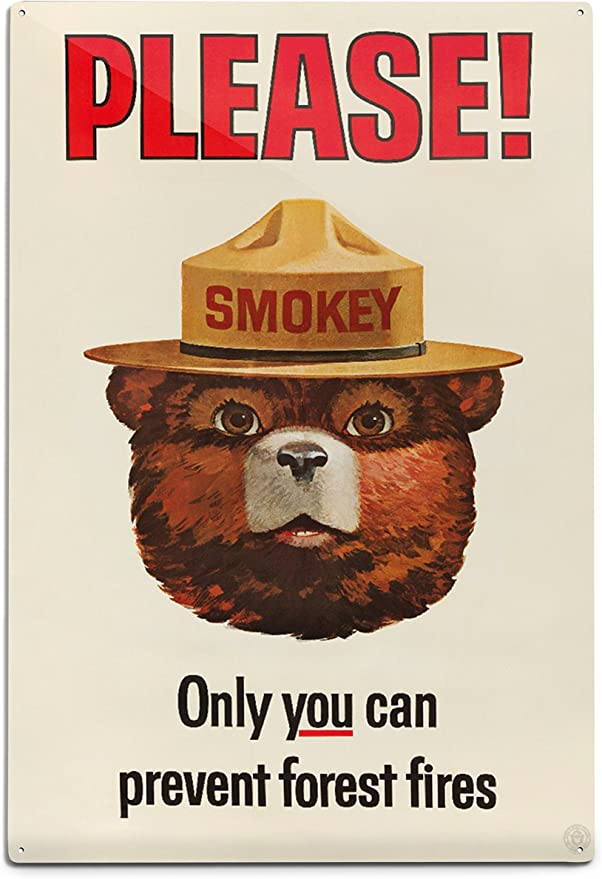
\includegraphics[width=0.3\textwidth]{images/smokeybear.jpg}
\end{center}

\end{frame}



\begin{frame}
\frametitle{Be Realistic}

Action items have to be realistic...\\
\quad Probably cannot say rewrite all code in Rust.

Not every report results in major head-exploding conclusions.

\end{frame}


\begin{frame}
\frametitle{Not Included In Report}

Avoid having:

\begin{itemize}
	\item Irrelevant detail
	\item Speculation
	\item Blaming
	\item Blaming
\end{itemize}


\end{frame}




\begin{frame}
\frametitle{Security, Report to the Bridge}

\begin{center}
	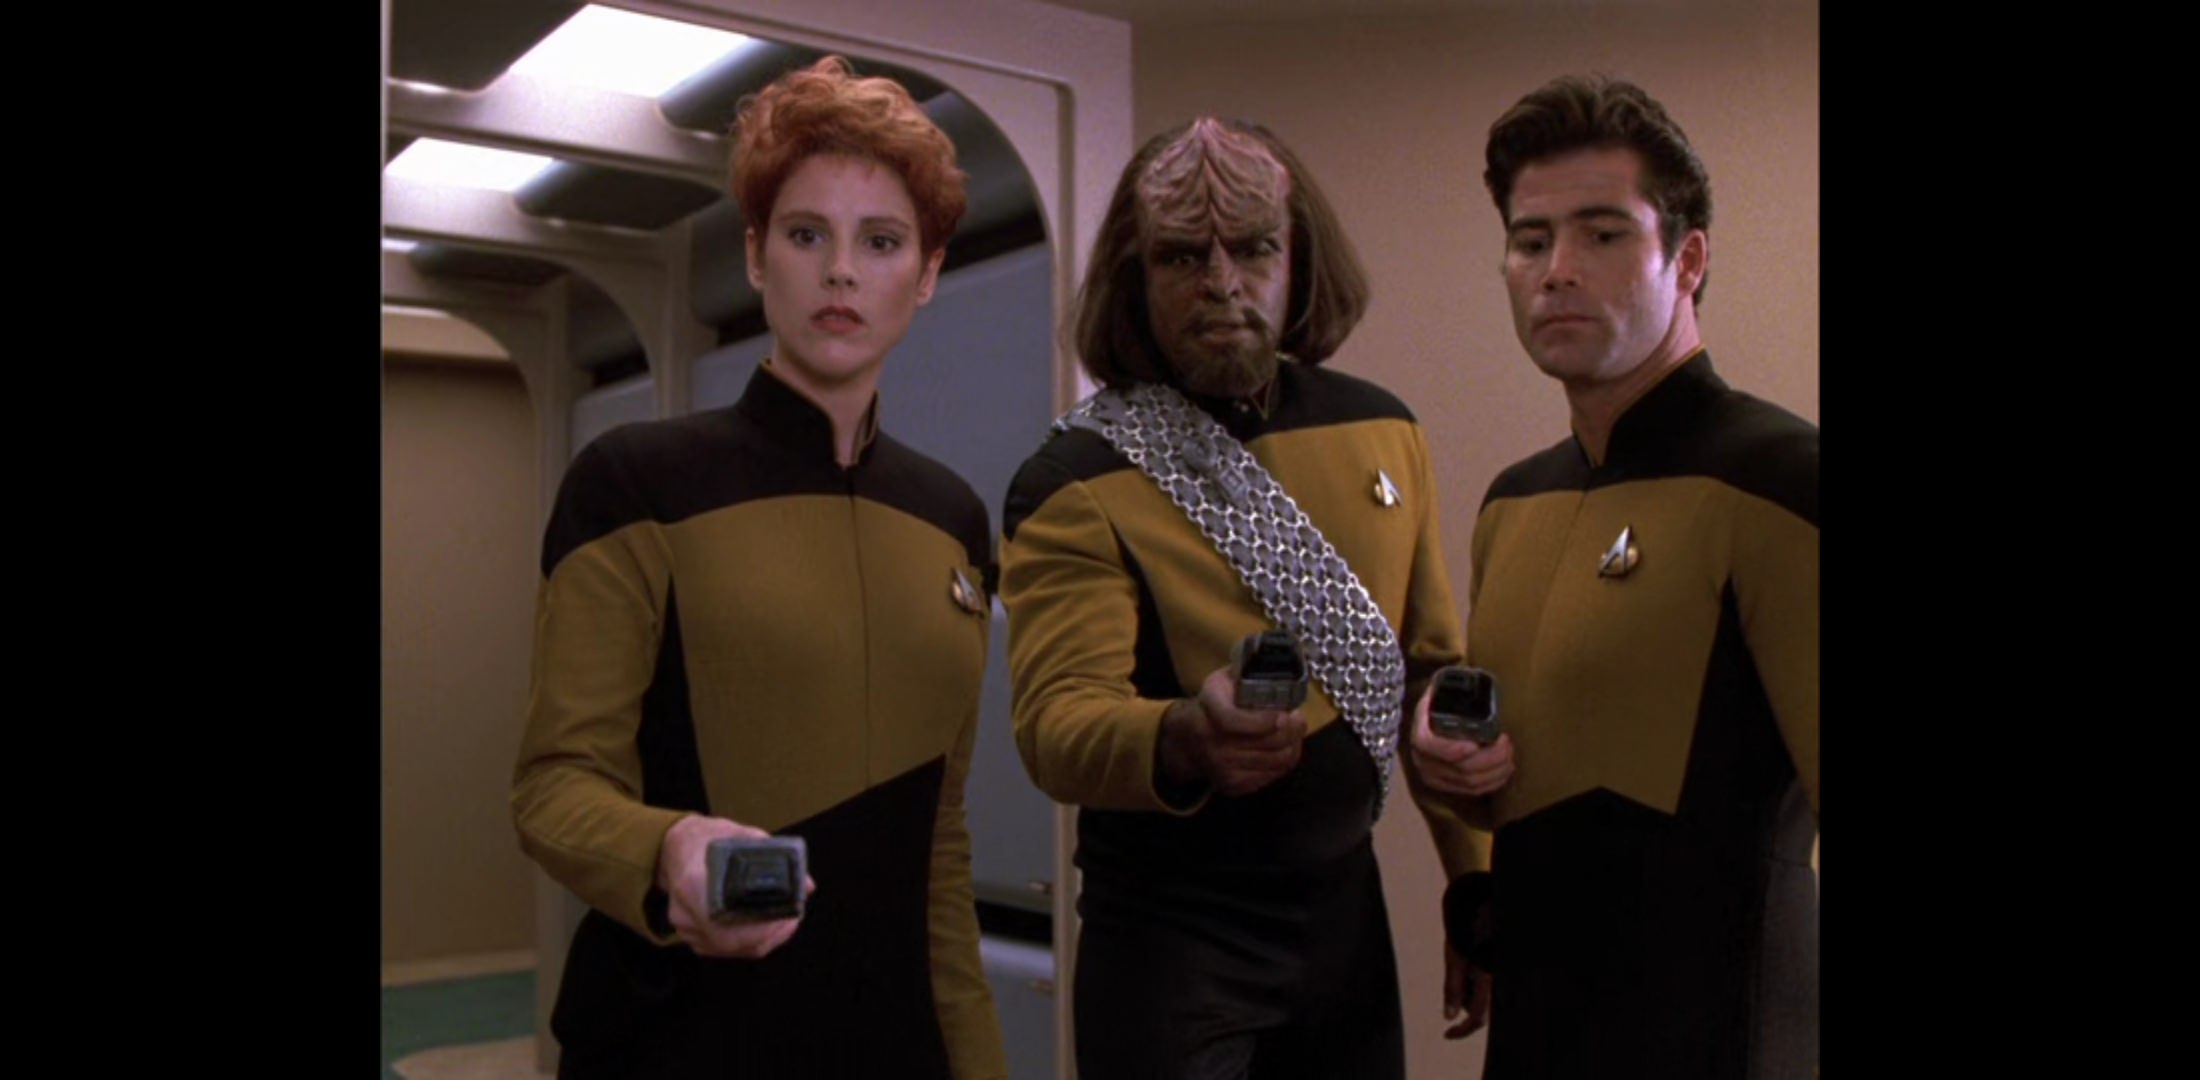
\includegraphics[width=\textwidth]{images/securityteam.jpg}
\end{center}

Having an always-available service accessible over the internet makes security a very big concern.

\end{frame}

\begin{frame}
\frametitle{Risk Enormous}

You can run some program with tons of security vulnerabilities offline and feel that the security problems can be managed. 

When it's online the risk is enormous. 

All kinds of vulnerabilities are a problem, but I'll call out two of them:

Code execution/injection and data leakage (information exposure). 


\end{frame}


\begin{frame}
\frametitle{Abusing Free Services for Fun and Profit}

Real-life attack about abusing free CPU time from cloud providers.

These are there for non-nefarious purposes but can be abused.

Also consider a scenario where attackers use your resources!

\end{frame}


\begin{frame}
\frametitle{Abusing Free Services for Fun and Profit}

Bypass signup limitations, browser scripting.

Mining cryptocurrency -- inefficiently -- but works.


Using \$103~000 of resources produces one coin worth about \$137: 0.13\% return.\\
\quad Or free money from attacker POV.

\begin{center}
	
\includegraphics[width=0.5\textwidth]{images/freerealestate.jpg}
\end{center}

\end{frame}


\begin{frame}
\frametitle{Abusing Free Services for Fun and Profit}

Disguise what is happening: no container called \texttt{mine-crypto-lol}\\
\quad \texttt{linux88884474} instead.

Generate random Github action names.

Spotting crypto mining is easier because it's CPU intensive...\\
\quad What about spyware, sending secrets to extortion rings?


\end{frame}



\begin{frame}
\frametitle{Information Exposure}

Information Exposure is bad for your reputation and expensive.

GDPR infractions get expensive: \url{https://enforcementtracker.com/}

Fines are for things like insufficient technical measures.

\end{frame}


\begin{frame}
\frametitle{Fun Example}

Remember talking about logging in tracing? Logging PII there was a big risk!

An example of a security process backfiring.


\end{frame}



\begin{frame}
\frametitle{Audit This}

There are some companies out there that will check your code for libraries with versions having known security vulnerabilities.

Sadly, when there is an updated version of a library, there may be breaking changes in it...

Checking for vulnerabilities should be an automatic process as part of your build and release procedures. 

\end{frame}


\end{document}

